\documentclass{beamer}
\usetheme{Madrid} % Clean theme
\usepackage{listings}
\usepackage{xcolor}
\usepackage{graphicx}

\usepackage{gvv}

% Code listing style
\lstset{
  basicstyle=\ttfamily\footnotesize,
  keywordstyle=\color{blue},
  stringstyle=\color{orange},
  commentstyle=\color{green!60!black},
  breaklines=true,
  frame=single,
  showstringspaces=false
}

\title{MatGeo Assignment - Problem 1.9.13}
\author{EE25BTECH11024}
\institute{IIT Hyderabad}

\begin{document}

% Title slide
\begin{frame}
  \titlepage
\end{frame}

% Problem statement
\begin{frame}{Problem Statement}
If $\vec{A}, \vec{B}, \vec{C}, \vec{D}$ are the points with position vectors $\hat{i}+\hat{j}-\hat{k}$, $2\hat{i}-\hat{j}+3\hat{k}$, $2\hat{i}-3\hat{k}$, $3\hat{i}-2\hat{j}+\hat{k}$ respectively, find the projection of AB along CD.
\end{frame}

% Solution using Rank Criterion (Slide 1)
\begin{frame}{Given Data:}
\noindent
\begin{center}
    \begin{tabular}{|c|c|c|}
    \hline
    \textbf{Symbol} & \textbf{Value} & \textbf{Description}  \\
    \hline
    \textbf{\vec{A}}      & \myvec{1 \\ 1\\-1}         & First Point\\
    \hline
    \textbf{\vec{B}}      & \myvec{2 \\ -1 \\3}        & Second Point\\
    \hline
    \textbf{\vec{C}}      & \myvec{2 \\ 0 \\-3}        &Third Point \\
    \hline
    \textbf{\vec{D}}      & \myvec{3 \\ -2 \\1}        &Fourth Point \\
    \hline
    \end{tabular}
\end{center}
\noindent
\end{frame}

\begin{frame}{Formula Used}
    The Projection of A along B is given by
    \begin{align}
    \vec{C} = \frac{\vec{A}^\top\vec{B}}{\|\vec{B}\|^2} \vec{B}
    \label{eq:2.4.19.1}
\end{align}
    
\end{frame}

\begin{frame}{Solution: }
\noindent
From the the given points we find AB and CD
\begin{align}
\vec{B} - \vec{A} = \myvec{1 \\ 2 \\-4}, \vec{D} - \vec{C} = \myvec{1 \\ 2 \\-4}
\label{eq:2.4.19.1}
\end{align}

Let P be the projection of AB along CD. We know that
\begin{align}
    \vec{P} = (\frac{(\vec{B} - \vec{A})^\top (\vec{D} - \vec{C})}{\|\vec{D} - \vec{C}\|^2}) (\vec{D} - \vec{C})
    \label{eq:2.4.19.2}
\end{align}

Substituting \eqref{eq:2.4.19.1} in \eqref{eq:2.4.19.2} we get
\begin{align}
    P = (\vec{D} - \vec{C}) =  \myvec{1 \\ 2 \\-4}
\end{align}

\end{frame}

\begin{frame}{Final Answer}
  Thus, the projection of AB along CD = $\myvec{1 \\ 2 \\-4}\\$

See Figure~\ref{fig:3DVectors}.   
\end{frame}

\begin{frame}{Figure}
    \begin{figure}[h!]
    \centering
    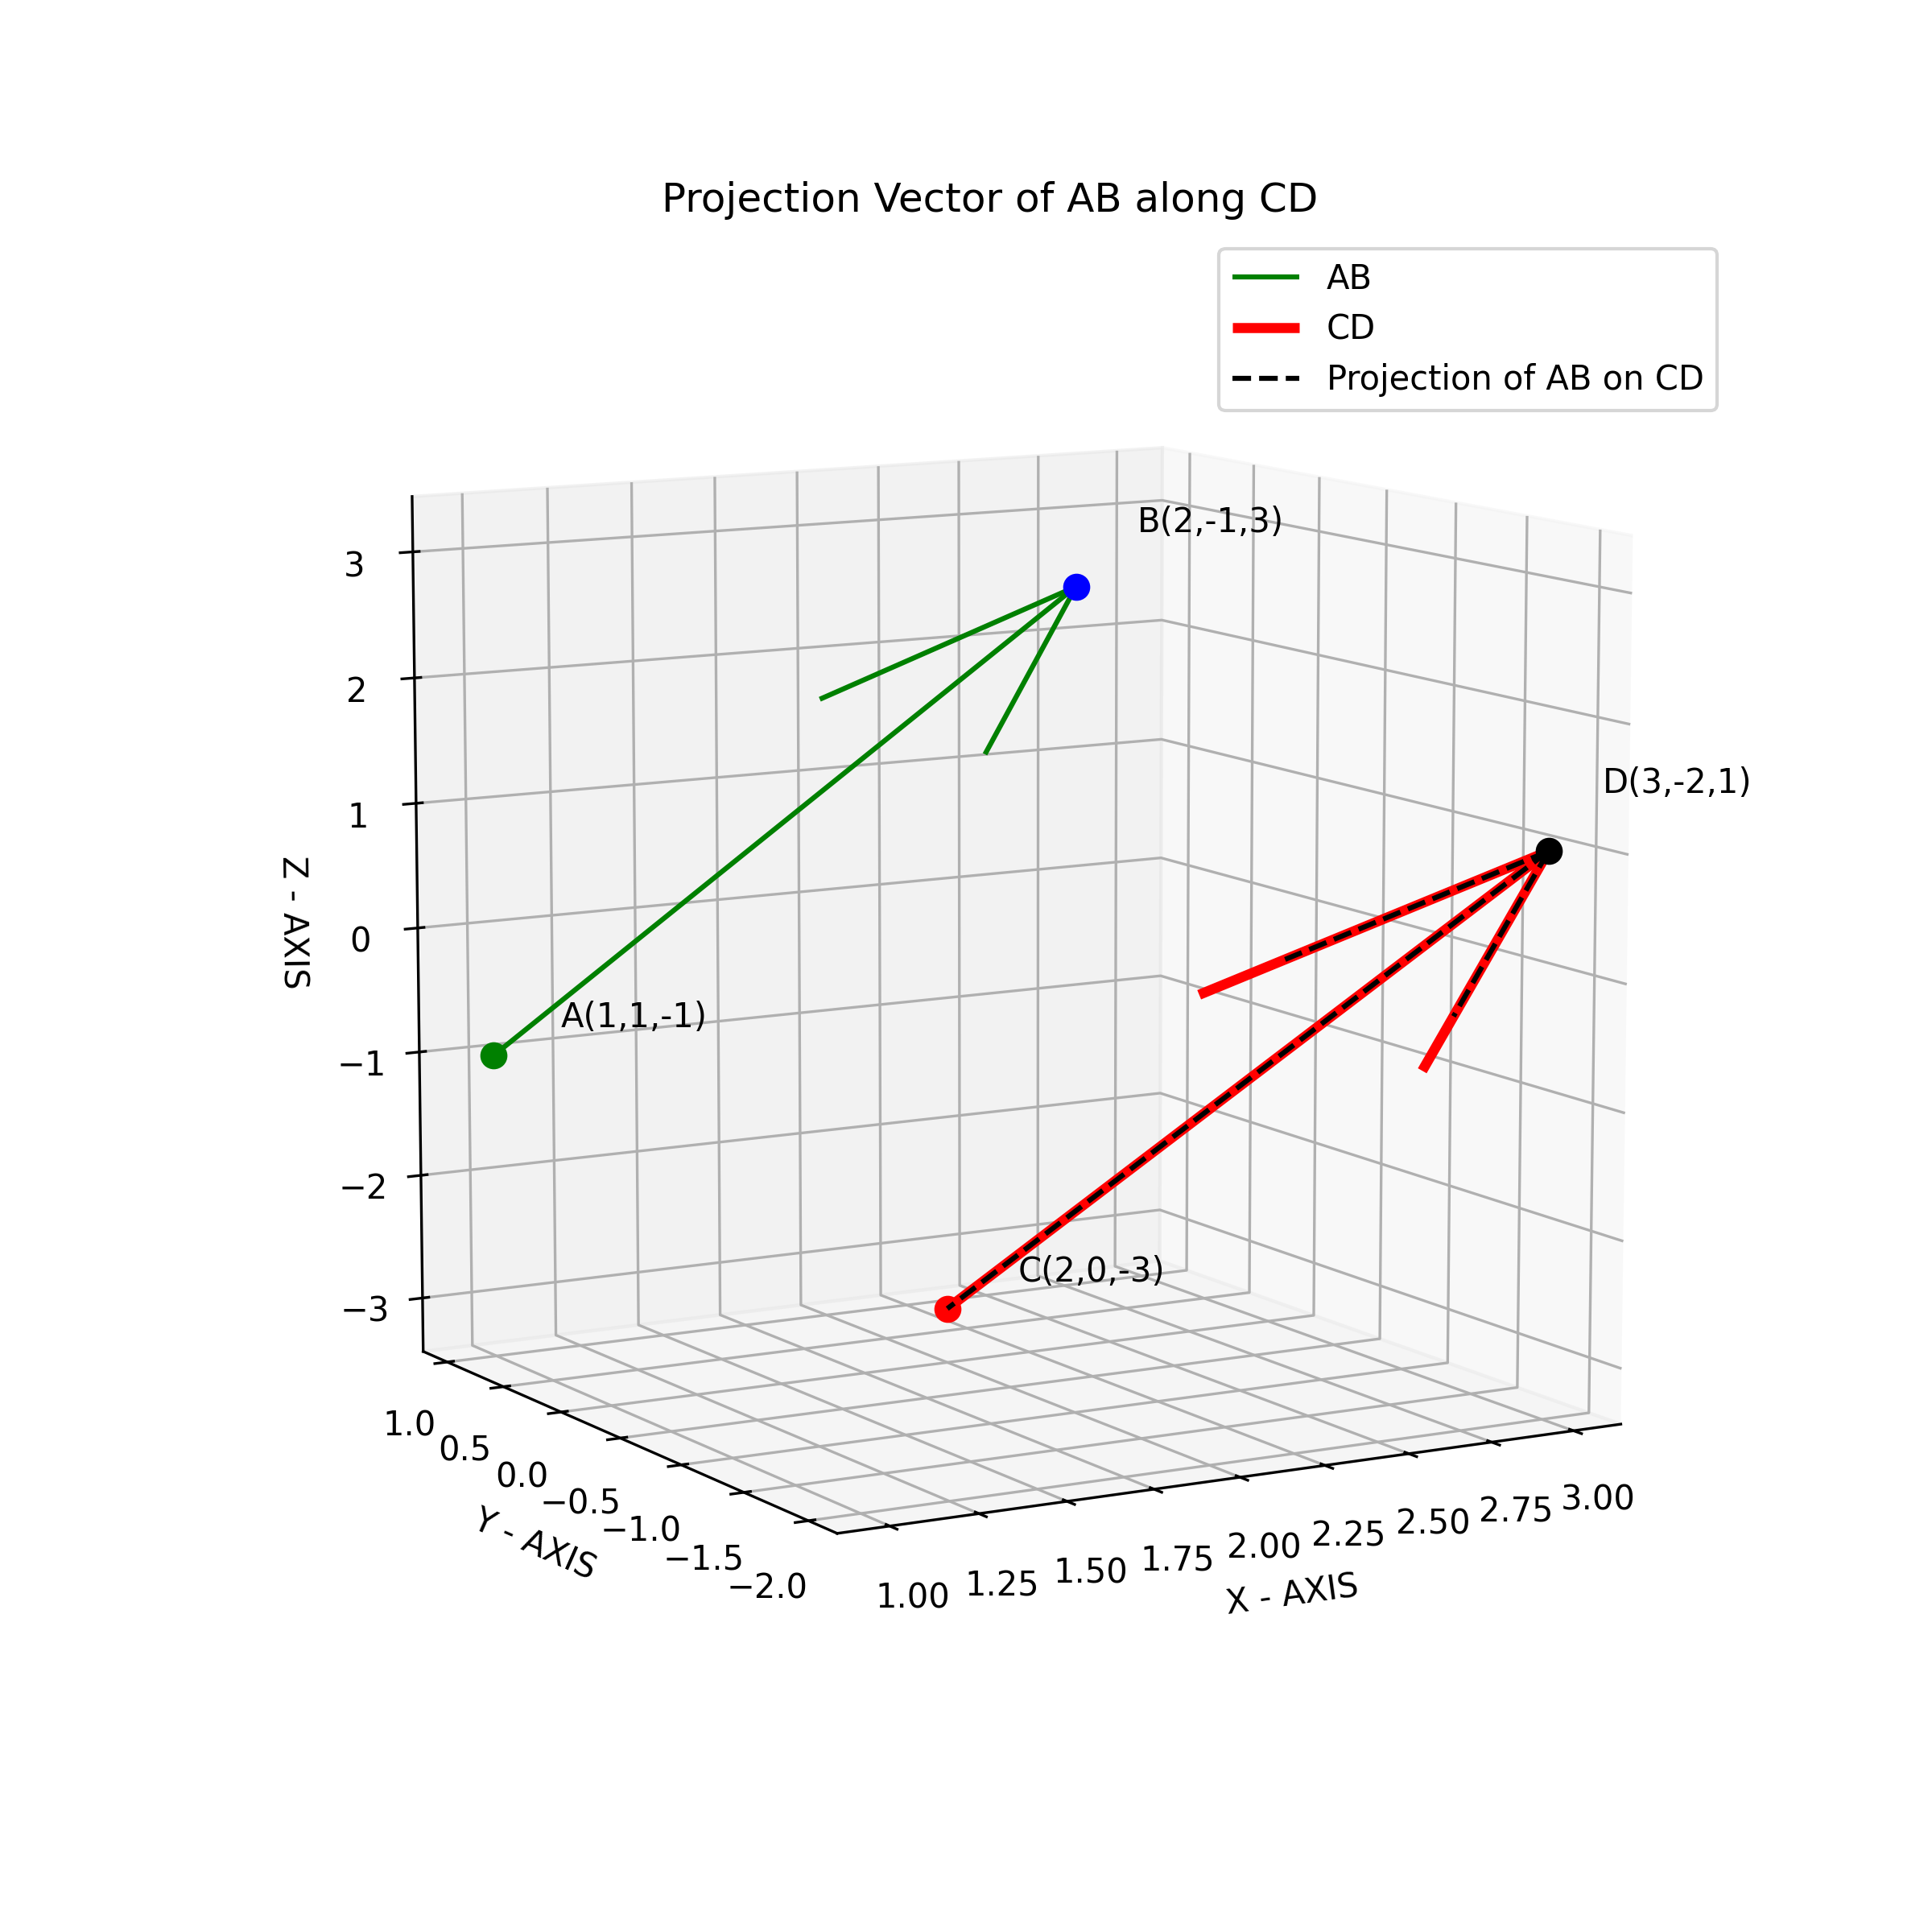
\includegraphics[width=0.7\linewidth]{figs/fig.png}
    \caption{}
    \label{fig:3DVectors}
\end{figure}
\end{frame}

% Python code 1
\begin{frame}[fragile]{Python Code: plot.py (Native)}
\begin{lstlisting}[language=Python]
import numpy as np
import matplotlib.pyplot as plt
from mpl_toolkits.mplot3d import Axes3D

A = np.array([1,1,-1])
B = np.array([2,-1,3])
C = np.array([2,0,-3])
D = np.array([3,-2,1])

fig = plt.figure(figsize = (8,8))
ax = fig.add_subplot(111, projection = '3d')

ax.quiver(A[0], A[1], A[2], B[0]-A[0], B[1]-A[1], B[2]-A[2], color = 'g', label = 'AB')
ax.quiver(C[0], C[1], C[2], D[0]-C[0], D[1]-C[1], D[2]-C[2], color = 'r', label = 'CD')
\end{lstlisting}
\end{frame}


\begin{frame}[fragile]{Python Code (Native Implementation – plot.py)}
\begin{lstlisting}[language=Python]
ax.scatter(*A, color='green', s=50)
ax.scatter(*B, color= 'blue', s=50)
ax.scatter(*C, color= 'red', s=50)
ax.scatter(*D, color= 'black', s=50)

ax.text(A[0]+0.1, A[1]-0.3, A[2]+0.3, "A(1,1,-1)")
ax.text(B[0]+0.3, B[1]+0.3, B[2]+0.3, "B(2,-1,3)")
ax.text(C[0]+0.1, C[1]-0.3, C[2]+0.3, "C(2,0,-3)")
ax.text(D[0]+0.3, D[1]+0.3, D[2]+0.3, "D(3,-2,1)")


ax.set_xlabel("X - AXIS")
ax.set_ylabel("Y - AXIS")
ax.set_zlabel("Z - AXIS")
ax.set_title("Vectors AB and CD in 3D Space")
\end{lstlisting}
\end{frame}

\begin{frame}[fragile]{Python Code (Native Implementation – plot.py)}
\begin{lstlisting}[language=Python]
ax.legend()
ax.set_box_aspect([1, 1, 1])  
ax.view_init(elev=10, azim=-120)
plt.savefig("fig3.png", dpi=300)
plt.show()
\end{lstlisting}
\end{frame}

\begin{frame}[fragile]{C Code (Shared Library – findprojection.c)}
\begin{lstlisting}[language=C]
#include <stdio.h>

void find_projection(double *A, double *B, double *C, double *D, double *projection){

double AB[3];
for (int i = 0; i < 3; i++) {
    AB[i] = B[i] - A[i];
}
double CD[3];
for (int i=0; i<3; i++){
    CD[i] = D[i] - C[i];
}

double dot_product = 0.0;
for (int i=0; i<3; i++) {
    dot_product += AB[i]*CD[i];
}
\end{lstlisting}
\end{frame}

\begin{frame}[fragile]{C Code (Shared Library – findprojection.c)}
\begin{lstlisting}[language=C]
double mag_square = 0.0;
for (int i=0; i<3; i++) {
mag_square += CD[i]*CD[i];
}

if (mag_square == 0) {
        projection[0] = 0;
        projection[1] = 0;
        projection[2] = 0;
        return;
    }
for (int i=0; i<3; i++){
    projection[i] = (dot_product/mag_square)*CD[i];
}

}
\end{lstlisting}
\end{frame}

% Python code 2
\begin{frame}[fragile]{Python Code: call.py (C + Python)}
\begin{lstlisting}[language=Python]
import ctypes
import numpy as np
import matplotlib.pyplot as plt
from mpl_toolkits.mplot3d import Axes3D

so = ctypes.CDLL("./find_projection.so")

so.find_projection.argtypes = [ctypes.POINTER(ctypes.c_double), ctypes.POINTER(ctypes.c_double), ctypes.POINTER(ctypes.c_double), ctypes.POINTER(ctypes.c_double), ctypes.POINTER(ctypes.c_double)]
so.find_projection.restype = None

A = np.array([1, 1, -1], dtype=np.double)
B = np.array([2, -1, 3], dtype=np.double)
C = np.array([2, 0, -3], dtype=np.double)
D = np.array([3, -2, 1], dtype=np.double)
\end{lstlisting}
\end{frame}

\begin{frame}[fragile]{Python Code (C Integrated – call.py)
}
\begin{lstlisting}[language=Python]
A_ptr = A.ctypes.data_as(ctypes.POINTER(ctypes.c_double))
B_ptr = B.ctypes.data_as(ctypes.POINTER(ctypes.c_double))
C_ptr = C.ctypes.data_as(ctypes.POINTER(ctypes.c_double))
D_ptr = D.ctypes.data_as(ctypes.POINTER(ctypes.c_double))

proj_result = (ctypes.c_double*3)()

so.find_projection(A_ptr, B_ptr, C_ptr, D_ptr, proj_result)
proj_vec = np.array(proj_result)

fig = plt.figure(figsize = (8,8))
ax = fig.add_subplot(111, projection = '3d')

ax.quiver(A[0], A[1], A[2], B[0]-A[0], B[1]-A[1], B[2]-A[2], color = 'g', label = 'AB')
ax.quiver(C[0], C[1], C[2], D[0]-C[0], D[1]-C[1], D[2]-C[2], color = 'r', label = 'CD', linewidth=3, arrow_length_ratio=0.4)
ax.quiver(C[0], C[1], C[2], proj_vec[0], proj_vec[1], proj_vec[2], color='black', linestyle = '--', label='Projection of AB on CD')
\end{lstlisting}
\end{frame}

\begin{frame}[fragile]{Python Code (C Integrated – call.py)
}
\begin{lstlisting}[language=Python]
ax.scatter(*A, color='green', s=50)
ax.scatter(*B, color= 'blue', s=50)
ax.scatter(*C, color= 'red', s=50)
ax.scatter(*D, color= 'black', s=50)

ax.text(A[0]+0.1, A[1]-0.3, A[2]+0.3, "A(1,1,-1)")
ax.text(B[0]+0.3, B[1]+0.3, B[2]+0.3, "B(2,-1,3)")
ax.text(C[0]+0.1, C[1]-0.3, C[2]+0.3, "C(2,0,-3)")
ax.text(D[0]+0.3, D[1]+0.3, D[2]+0.3, "D(3,-2,1)")
\end{lstlisting}
\end{frame}

\begin{frame}[fragile]{Python Code (C Integrated – call.py)
}
\begin{lstlisting}[language=Python]
ax.set_xlabel("X - AXIS")
ax.set_ylabel("Y - AXIS")
ax.set_zlabel("Z - AXIS")
ax.set_title("Projection Vector of AB along CD")

ax.legend()
ax.set_box_aspect([1, 1, 1])  
ax.view_init(elev=10, azim=-120)
plt.savefig("fig3'.png", dpi=300)
plt.show()
\end{lstlisting}
\end{frame}



\end{document}


